\documentclass[../../topologia_algebraica]{subfiles}
\begin{document}
\section{Variedades}\label{sec:variedades}

En esta secci\'on, desarrollar\'e la teor\'ia de espacios topol\'ogicos que localmente son
euclideanos. La idea es pegar conjuntos abiertos de un $\RR^n$ mediante difeomorfismos
(definir\'e este concepto m\'as adelante): si $U_1$ y $U_2$ son conjuntos abiertos de $\RR^n$
con subconjuntos abiertos $W_i\subseteq U_i$ tales que hay un difeomorfismo $f:W_1\ra W_2$,
entonces puedo identificar $W_1$ con $W_2$ para obtener un nuevo espacio:

\begin{figure}[ht]%%%%%%%%%%%%%%%%%%%%%%%%%%%%%%%%%%%%%%%%%%%%%%%%%%%%%%%%%%% FIGURA
  \centering
  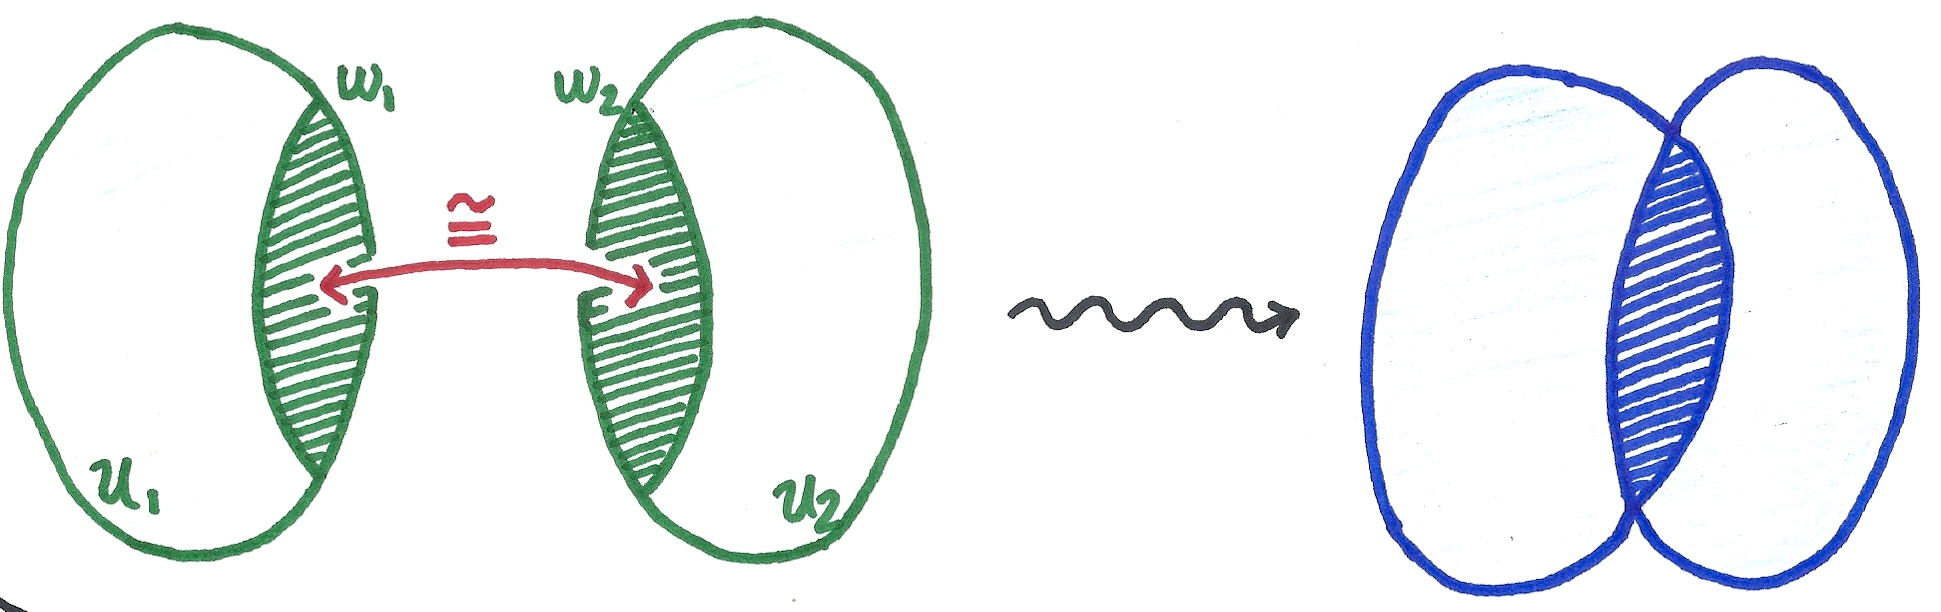
\includegraphics[scale=0.13]{pegado_difeomorfismo}
\end{figure}%%%%%%%%%%%%%%%%%%%%%%%%%%%%%%%%%%%%%%%%%%%%%%%%%%%%%%%%%%%%%%%%%%%%%%%%%%

\noindent Hago m\'as preciso esta idea con la siguiente lista de definiciones:

\begin{defin}
  Sea $M$ un espacio paracompacto%
  \footnote{Un espacio $X$ es paracompacto si toda cualquier cubierta abierta
    $\Uu=\{U_j\}_{j\in J}$ de $X$ admite un refinamiento localmente finita, ie. que para todo
    punto $x\in X$, existe una vecindad $V\subseteq X$ de $x$ que intersecta s\'olo una
    cantidad finita de abiertos del refinamiento.}
  (en particular es Hausdorff). Defino que $M$ es un \emph{variedad topol\'ogica} si para toda
  $x\in M$, existe una vecindad $U\subseteq M$ alrededor de $x$ y un homeomorfismo
  $\varphi:U\ra V$ donde $V\subseteq\RR^n$ es un conjunto abierto. A veces $M$ se denota por
  $M^n$ para determinar a qu\'e espacio euclideano se parece $M$ localmente.
  La pareja $(U,\varphi)$ es una \emph{carta} de $M$ alrededor de $x$ y si
  $\Phi=\{(U_{\la},\varphi_{\la})\}_{\la\in\Lambda}$ es una familia de cartas de $M$ tales que
  $M=\cup U_{\la}$, se dice que $\Phi$ es un \emph{atlas} de $M$.
\end{defin}
\begin{figure}[ht]%%%%%%%%%%%%%%%%%%%%%%%%%%%%%%%%%%%%%%%%%%%%%%%%%%%%%%%%%%% FIGURA
  \centering
  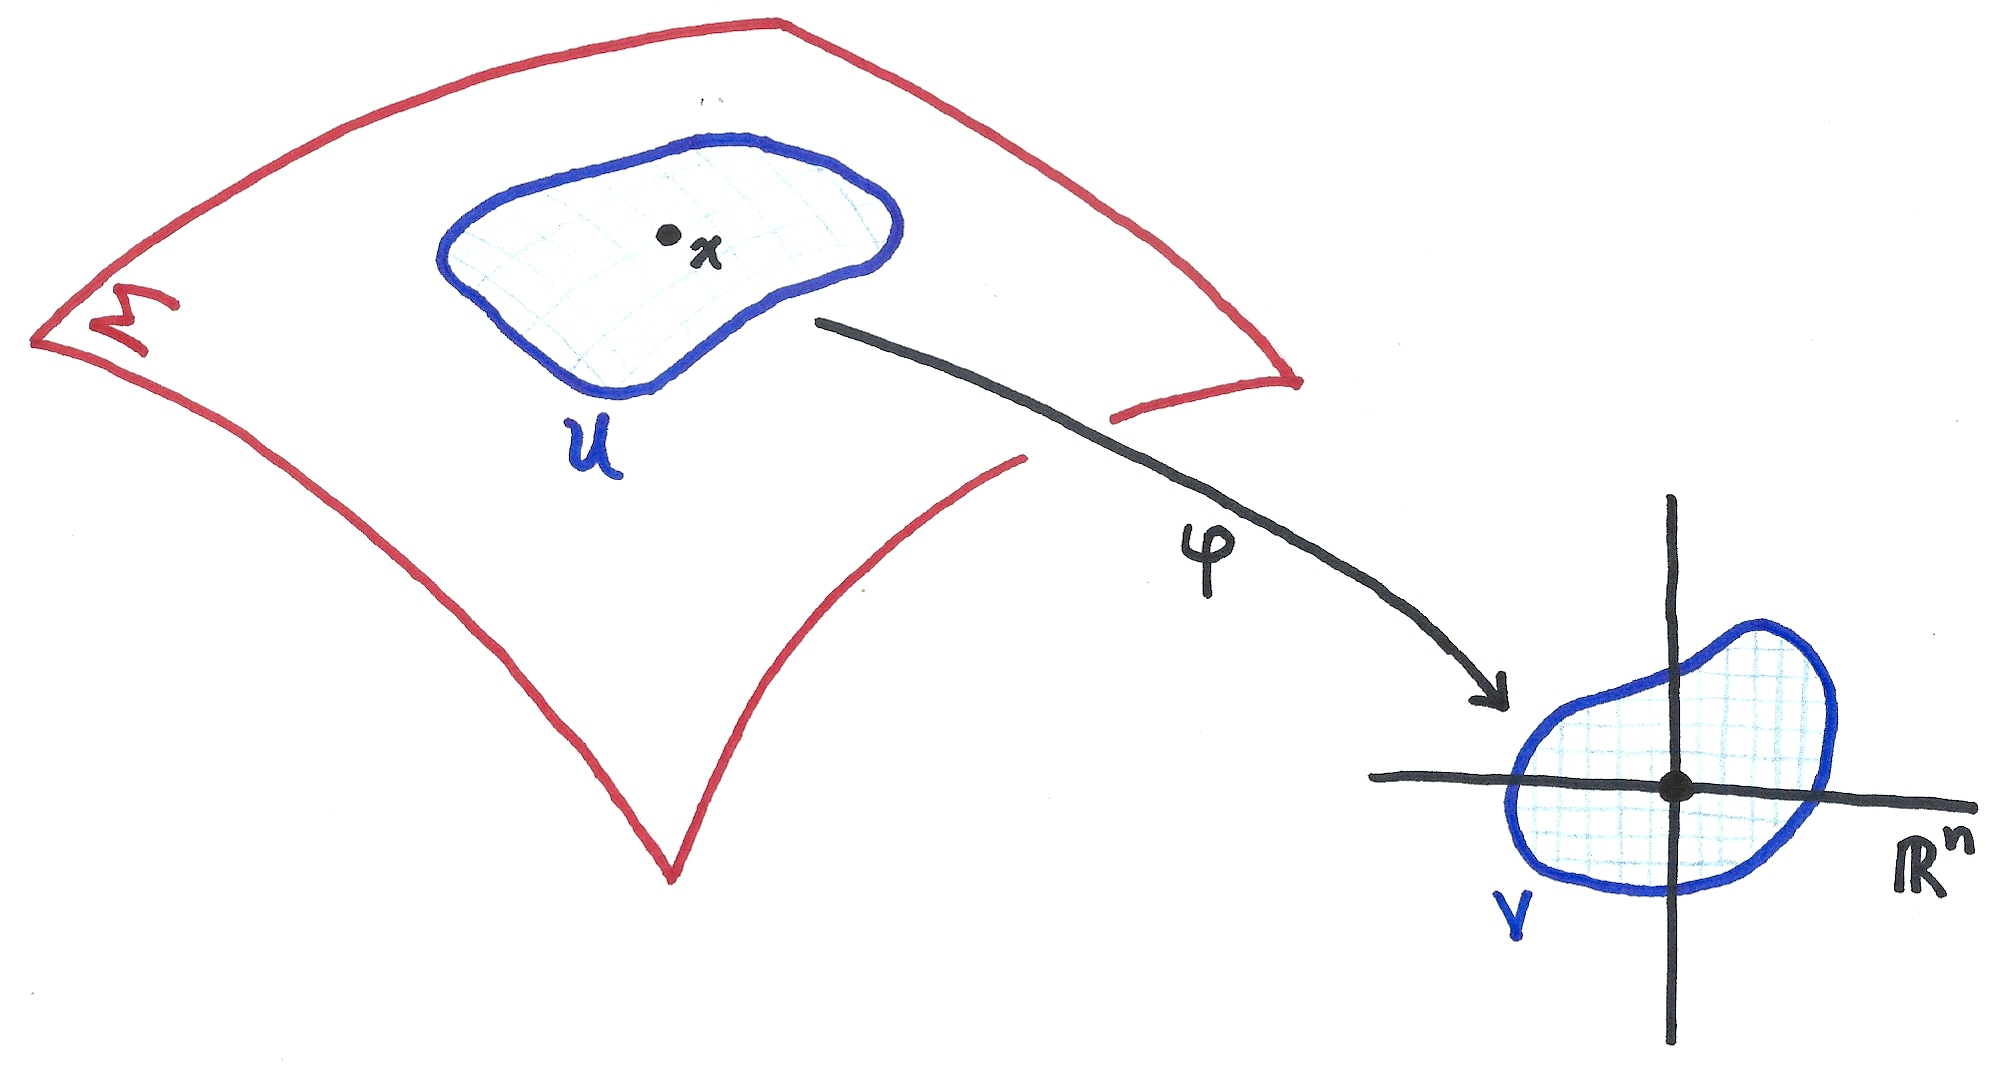
\includegraphics[scale=0.12]{variedad_topologica}
\end{figure}%%%%%%%%%%%%%%%%%%%%%%%%%%%%%%%%%%%%%%%%%%%%%%%%%%%%%%%%%%%%%%%%%%%%%%%%%%

La estructura diferenciable de $\RR^n$ la codifico en una variedad topol\'ogica a trav\'es
del atlas:

\begin{defin}
  Sea $\Phi=\{(U_{\la},\varphi_{\la})\}_{\la\in\Lambda}$ un atlas de una variedad topol\'ogica
  $M$. El atlas $\Phi$ es un \emph{atlas suave} (ie. de clase $C^{\infty}$) si para cualesquiera
  $\la,\mu\in\Lambda$ tales que $U_{\la}\cap U_{\mu}\neq\emptyset$ se cumple que
  \[
    \varphi_{\la}\circ\varphi_{\mu}^{-1}:
    \varphi_{\mu}\big[U_{\la}\cap U_{\mu}\big]\ra\varphi_{\la}\big[ U_{\la}\cap U_{\mu} \big]
  \]
  es una funci\'on de clase $C^{\infty}$. La funci\'on
  $\varphi_{\mu\la}:=\varphi_{\la}\circ\varphi_{\mu}^{-1}$ se llama el \emph{cambio de coordenadas}
  de la carta $(U_{\mu},\varphi_{\mu})$ a la carta $(U_{\la},\varphi_{\la})$
  (v\'ease la figura \ref{fig:atlas_suave}). En otras palabras,
  el atlas $\Phi$ es suave si todos sus cambios de coordenadas son suaves.
\end{defin}
\begin{figure}[ht]\label{fig:atlas_suave}%%%%%%%%%%%%%%%%%%%%%%%%%%%%%%%%%%%%%%%%%%%%%%%%%% FIGURA
  \centering
  \caption{Representaci\'on gr\'afica de los cambios de coordenadas de un atlas.}
  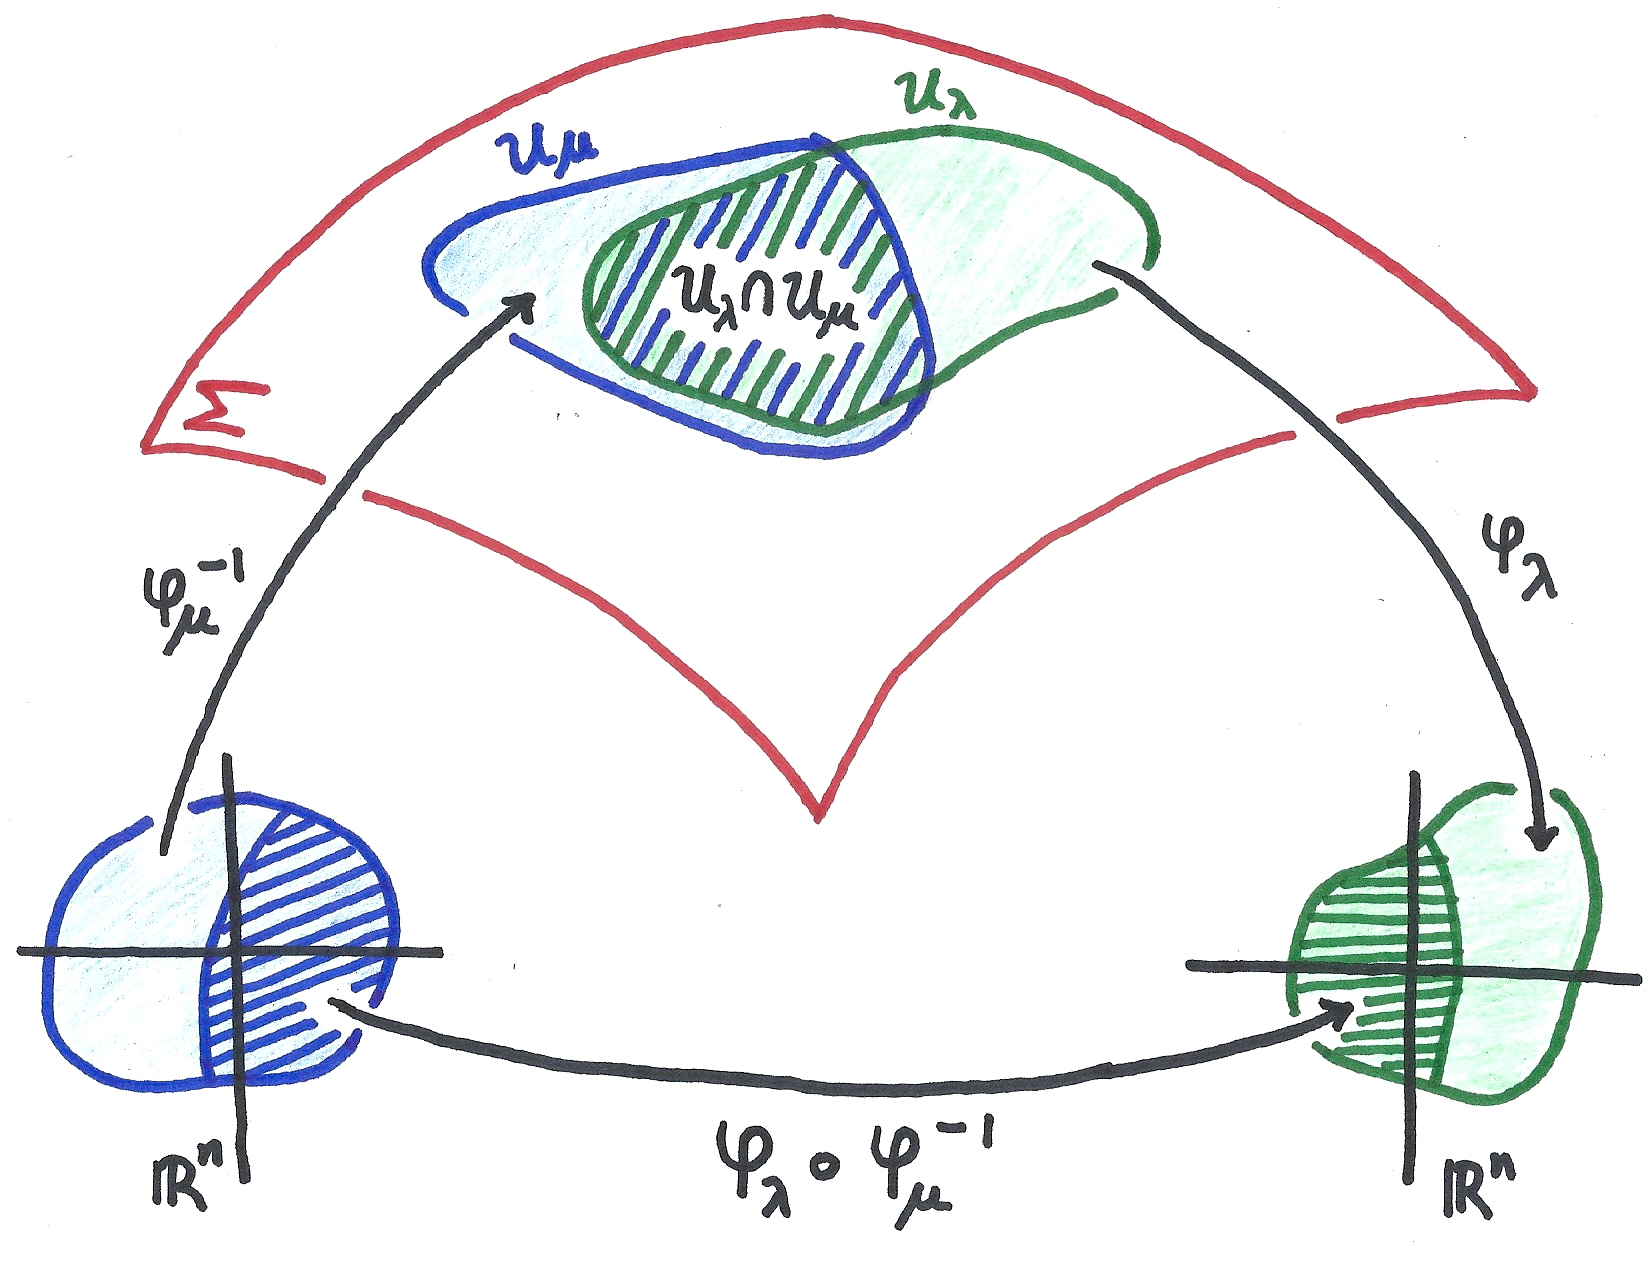
\includegraphics[scale=0.12]{atlas_suave}
\end{figure}%%%%%%%%%%%%%%%%%%%%%%%%%%%%%%%%%%%%%%%%%%%%%%%%%%%%%%%%%%%%%%%%%%%%%%%%%%

Observa que estudiar la diferenciablididad de $\varphi_{\mu\la}$ tiene sentido porque su dominio
$\varphi_{\mu}[U_{\la}\cap U_{\mu}]$  y su contradominio $\varphi_{\la}\big[U_{\la}\cap U_{\mu}\big]$
son subconjuntos abiertos de $\RR^n$.

\begin{defin} Sea $\Phi$ un atlas suave de una variedad topol\'ogica $M$. El atlas $\Phi$
  es una \emph{estructura diferenciable} de $M$ si $\Phi$ es maximal, es decir para toda
  carta arbitraria $(U,\psi)$ que cumple que
  \[
    \varphi\circ\psi^{-1} \quad\text{y}\quad \psi\circ\varphi^{-1}\quad\text{son suaves}\quad
    \forall \; (V,\varphi)\in\Phi,
  \]
  entonces necesariamente $(U,\psi)\in\Phi$.
\end{defin}

La maximalidad de un atlas $\Phi$ dice que toda carta $(U,\psi)$ compatible con todas las cartas de
$\Phi$ (ie. que los cambios de coordenadas sean suaves) tiene que ser un elemento de $\Phi$.
Intuitivamente, esto significa que a $\Phi$, ya se le ha agregado todas las posibles cartas
compatibles. Observa que cualquier atlas $\Phi$ se puede acompletar a un atlas maximal, simplemente
agregandole todas las posibles cartas compatibles. En la pr\'actica trabajar\'e con atlas peque\~nas
(finitas) y cuando hablo de la estructura diferenciable inducida por estos atlas, me refiero
t\'acitamente al atlas maximal que genera el atlas peque\~no.

\begin{defin}
  Una \emph{variedad diferenciable} es una pareja $(M,\Phi)$ donde $M$ es una variedad topol\'ogica
  y $\Phi$ es una estructura diferenciable.
\end{defin}

Ahora analizo unos ejemplos importantes de variedades diferenciables:
\begin{ejemplo}\label{ejemplo:estructura_diferenciable_canonica_Rn}
  ($\RR^n$) Defino $\iota=\{(\RR^n,\Id)\}$ que claramente es un atlas suave porque $\Id:\RR^n\ra\RR^n$
  es un homeomorfismo (suave). Entonces si $\iota'$ es el atlas maximal generado por $\iota$ tengo que
  $(\RR^n,\iota')$ es una variedad diferenciable. A esta estructura diferenciable la llamo la
  \emph{estructura diferenciable can\'onica} de $\RR^n$.
\end{ejemplo}

\begin{ejemplo}
  ($\Sn^n$) Primero observa que cualquier atlas de $\Sn^n$ debe tener m\'as de una carta porque si
  tuviera solamente una, ie. $(\Sn^n,\varphi)$, entonces $\varphi$ ser\'ia un homeomorfismo entre
  $\Sn^n$ y un abierto de $\RR^n$, pero esto no puede suceder porque $\Sn^n$ es compacto. Por lo
  tanto cualquier atlas de $\Ss^n$ debe tener al menos dos cartas. A continuaci\'on construyo dos
  atlas para $\Sn^n$:

  Primero defino dos abiertos que cubren a $\Sn^n\subset\RR^{n+1}$. Sean
  $U_{\pm}:=\Sn^n-\{0,\ldots,0,\pm 1\}$, es decir $U_+$ es la esfera menos el polo norte y $U_-$ es la
  esfera menos el polo sur. Ahora defino:
  \[
    \varphi_{\pm}:U_{\pm}\lra \RR^n \quad\text{con}\quad
    \varphi_{\pm}(x_1,\ldots,x_{n+1})=\paren{\frac{x_1}{1\mp x_{n+1}},\ldots,\frac{x_n}{1\mp x_{n+1}}}=
    \frac{1}{1\mp x_{n+1}}(x_1,\ldots,x_n).
  \]

  \import{\directory}{/ejercicios/17}%%%%%%%%%%%%%%%%%%%%%%%%%%%%%%%%%%%%%%%%%%%%%%%%% EJERCICIO 17
  
  A  estas cartas se les llaman \emph{proyecciones estereogr\'aficas}: en general la funci\'on
  $\varphi_+$ le asigna a $x\in\Sn^n$ el punto de intersecci\'on del subespacio
  $\RR^n\times\{0\}\subset\RR^{n+1}$ con la recta que une el polo norte con $y\in\Sn^n$:

  De hecho esta construcci\'on es lo que me permiti\'o darle una f\'ormula expl\'icita a las
  funciones inversas de las proyecciones estereogr\'aficas: parametriz\'e el segmento de recta que
  empieza en el polo norte, y termina en un punto $x\in\RR^n=\RR^n\times\{0\}\subset\RR^{n+1}$,
  despu\'es calcul\'e el valor del par\'ametro para que me de un punto sobre la esfera. Resumo
  este proceso en el siguiente dibujo:
  \begin{figure}[ht]%%%%%%%%%%%%%%%%%%%%%%%%%%%%%%%%%%%%%%%%%%%%%%%%%%%%%%%%%%% FIGURA
    \centering
    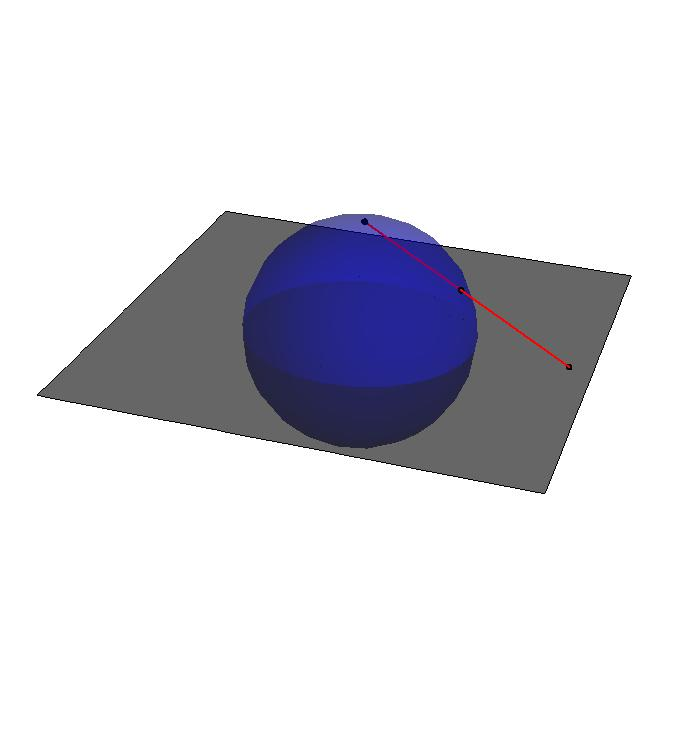
\includegraphics[trim=0 200 0 200, clip,scale=0.35]{proyeccion_estereografica}
  \end{figure}%%%%%%%%%%%%%%%%%%%%%%%%%%%%%%%%%%%%%%%%%%%%%%%%%%%%%%%%%%%%%%%%%%%%%%%%%%
\end{ejemplo}

\begin{ejemplo}\label{ejemplo:cartas_hemisferios}($\Sn^n$)
  En la proposici\'on \ref{prop:smash_esferas} de la secci\'on \ref{sec:producto_smash} introduje
  las funciones $\rho_{\pm}$ que relacionaban los hemisferios
  de la esfera con el disco como subconjunto de $\RR^n$. Con estas funciones doy otro atlas para la
  esfera que resulta \'util (cambiar\'e un poco la notaci\'on): sea $\DD_n\subset\RR^n$ el disco
  unitario de radio 1 alrededor del 0 y sea $\overset{\circ}{\DD}$ el interior del disco y defino
  $V_i^{\pm}:=\{(x_1,\ldots,x_{n+1})\in\Sn^n\mid \pm x_i>0\}$ como los distintos hemisferios abiertos
  (de dimensi\'on $n$) de la esfera. Con esto escribo
  \[
    h_i^{\pm}:V_i^{\pm}\lra \overset{\circ}{\DD}  \quad\text{con}\quad
    h_i^{\pm}(x_1,\ldots,x_{n+1})=(x_1,\ldots,\widehat{x_i},\ldots,x_{n+1})
  \]
  donde la notaci\'on $\widehat{x_i}$ significa que omito esa coordenada del vector, es decir
  $(x_1,\ldots,\widehat{x_i},\ldots,x_{n+1})=(x_1,\ldots,x_{i-1},x_{i+1},\ldots,x_{n+1})$. Aqu\'i
  uso la letra $h$ para denotar ``hemisferio''.

  Como todo elemento $x=(x_1,\ldots,x_{n+1})\in\Sn^n$ tiene al menos una coordenada distinto de cero,
  por ejemplo $x_i$, entonces $x\in V_i^+$ o $x\in V_i^-$ y as\'i $\Sn^n=\cup V_i^{\pm}$ entonces
  $\Hh=\{(h_i^+V_i^+),(h_i^-,V_i^-)\}_{i=1}^{n+1}$ es un atlas con $2(n+1)$ cartas. En efecto, cada
  $h_i^{\pm}$ es un homeomorfismo porque las funciones:
  \[
    \rho_i^{\pm}:\overset{\circ}{\DD} \lra V_i^{\pm} \quad\text{con}\quad
    \rho_i^{\pm}(x_1,\ldots,x_n)=\paren{x_1,\ldots,x_{i-1},\pm\sqrt{1-\sum x_k^2},x_{i},\ldots,x_n}
  \]
  es el inverso de $h_i^{\pm}$ (ve la proposici\'on \ref{prop:smash_esferas} para ver porque
  $\rho_i^{\pm}$, y as\'i $h_i^{\pm}$, es un homeomorfismo). En otras palabras, $\rho_i^{\pm}$ inserta
  el t\'ermino $(\sum x_k^2)^{1/2}$ en la $i$-\'esimo lugar para obtener un vector en
  $\Sn^n\subset\RR^{n+1}$. Con esto tengo que $\rho_i^{\pm}=(h_i^{\pm})^{-1}$.

  El atlas $\Hh$ es suave porque para $i< j$ tengo:
  \begin{align*}
    h_i^{\pm}\circ (h_j^{\pm})^{-1}(x)& =
    h_i^{\pm}\circ \rho_j^{\pm}(x_1,\ldots,x_n)=
    h_i^+\paren{x_1,\ldots,x_{j-1},\pm\sqrt{1-\sum x_k^2},x_j,\ldots,x_n} \\ & =
    (x_1,\ldots,\widehat{x_i},\ldots,\pm\sqrt{1-\sum x_k^2},\ldots,x_n)
  \end{align*}
  que es claramente una funci\'on suave porque $\sum x_k^2\leq 1$ ya que $x$ es un elemento del disco
  unitario. Los otros casos $j>i$, $j=i$ o $h_j^{\mp}$ son equivalentes o triviales. Por lo tanto
  todos los cambios de coordenadas son suaves y as\'i $\Hh$ es un atlas suave.
\end{ejemplo}

He dado dos atlas para $\Sn^n$, $\Phi$ y $\Hh$, pero resulta que definen la misma estructura
diferenciable, entonces las variedades diferenciables $(\Sn^n,\Phi)$ y $(\Sn^n,\Hh)$ son exactamente
el mismo porque el atlas maximal que generan $\Phi$ y $\Hh$ son el mismo. Para probar esto, s\'olo
hay que probar que los cambios de coordenadas $\varphi_{\pm}\circ (h_i^{\pm})^{-1}$ y
$h_i^{\pm}\circ\varphi_{\pm}^{-1}$ son suaves y as\'i garantizamos que todas las cartas de $\Phi$ y
$\Hh$ son elementos del atlas maximal que generan ambos.

\import{\directory}{ejercicios/18} %%%%%%%%%%%%%%%%%%%%%%%%%%%%%%%%%%%%%%%%%%%%%%% EJERCICIO 18

\begin{ejemplo}($\RR$) Defino el atlas $\Theta$ con \'unica carta $(\RR,x\mapsto x^3)$. Claramente
  es un atlas porque $x\mapsto x^3$ es un homeomorfismo (con inverso $x\mapsto x^{1/3}$ que es
  continua). Adem\'as $\Theta$ es suave porque nada m\'as tiene una carta. A diferencia del ejemplo
  \ref{ejemplo:estructura_diferenciable_canonica_Rn} (con $n=1$), este atlas no es compatible
  con el atlas can\'onico $\iota$ de $\RR$:

  \import{\directory}{ejercicios/19} %%%%%%%%%%%%%%%%%%%%%%%%%%%%%%%%%%%%%%%%%%%%%% EJERCICIO 19
\end{ejemplo}

El atlas $\Hh$ de la esfera me permite definirle una estructura diferenciable sobre el espacio
pryectivo real:

\begin{defin}
  El \emph{espacio proyectivo real} de dimensi\'on $n$, denotado por $\RR P^n$ es el espacio
  cociente:
  \[
    \RR P^n:=\RR^{n+1}-\{0\}/_{\sim}
  \]
  donde $x\sim y$ si existe un escalar $\la>0$ tal que $x=\la y$. A la proyecci\'on can\'onica,
  la denoto por $p:(\RR^{n+1}-\{0\})\ra \RR P^n$.
\end{defin}

Observa que toda $x\in\RR^{n+1}-\{0\}$ cumple $[x]=[\|x\|^{-1}x]$, donde $\hat{x}:=\|x\|^{-1}x$
es un elemento de $\Sn^n$. Por lo tanto $[x_1]\neq[x_2]$ implica $[\|x_1\|^{-1}x_1]\neq[\|x_2\|^{-1}x_2]$ y
en particular $\hat{x_1}\neq\hat{x_2}$. Como $\Sn^n$ es Hausdorff, existen vecindades $U_1$ y $U_2$
que separan los $\hat{x_1}$ y $\hat{y_2}$ y as\'i $V_i=\{[z] \mid \hat{z}\in U_i\}$ son abiertos
de $\RR P^n$ que separan a $[x_1]$ de $[x_2]$: claramente $p[V_i]$ es el cono abierto generado
por todas las rectas que pasan por el origen y pasan por $V_i$ y si $[z]\in V_1\cap V_2$ entonces
$\hat{z}\in U_1\cap U_2=\emptyset$ por lo tanto $V_1\cap V_2=\emptyset$).

El proceso de tomar cocientes la podemos separar en dos: la idea es que estamos contrayendo
todas las rectas que pasan por el origen a puntos. Como cada recta de estas tienen dos
vectores directores unitarios, podemos primero contraer cada recta a dos puntos sobre la esfera
$\Sn^n\subset\RR^{n+1}-\{0\}$ y despues identificar ambos vectores directores. Si $x$ es un vector
unitario director de una recta, entonces $-x$ es el otro vector director unitario.

Estas ideas sugieren que el espacio proyectivo real de dimensi\'on $n$ es la esfera $\Sn^n$ m\'odulo
ant\'ipodas, es decir $x\sim -x$. De hecho, esto es verdadero:

\import{\directory}{ejercicios/20} %%%%%%%%%%%%%%%%%%%%%%%%%%%%%%%%%%%%%%%%%%% EJERCICIO 20

Esta nueva descripci\'on del espacio proyectivo nos permite darle una estructura diferenciable a
$\RR P^n$ con el atlas $\Hh$ de $\Sn^n$.

\begin{ejemplo}

Los dos hemisferios $V_i^+$ y $V_i^-$ se identifican bajo el cociente $\Sn^n/_{-x\sim x}$ porque
$x\in V_i^+\;\;\iff\;\; -x\in V_i^-$. Por lo tanto $q[V_i^+]=q[V_i^-]=:V_i$ es un abierto del
espacio proyectivo. Como las $V_i^{\pm}$ cubr\'ian a $\Sn^n$, entonces las $V_i$ cubren a $\RR P^n$.

Para toda $x\in\RR P^n$ tengo que $q^{-1}[x]=\{x,-x\}$ lo cual implica que $q$ es inyectiva
restringido a un conjunto $V\subseteq\Sn^n$ si y s\'olo si existen $x\in V \;\;\then\;\; -x\not\in V$.
Las $V_i^{\pm}$ cumplen esto ya que
\[
  x\in V_i^{\pm} \quad\then\quad
  m \pm x_i>0   \quad\then\quad
  \mp x_i<0    \quad\then\quad
  -x\not\in V_i^{\mp}
\]
Entonces la restricci\'on $q_i:=q|_{V_i^{+}}$ tiene inverso izquierdo. Lo llamo $\tilde{g}_i$.

Para cada $V_i\subset\RR P^n$ defino la carta $(V_i,h_i)$ como:
\[
  \begin{tikzcd}
    V_i^+ \arrow[r,"h_i^+"] \arrow[d,"q_i"] & \overset{\circ}{\DD} \\
    V_i \arrow[u,bend left,"\tilde{g}_i"] \arrow[ur,"h_i"'] & 
  \end{tikzcd}
\]
Claramente $h_i$ es un homeomorfismo. El atlas $\mathfrak{h}=\{(V_i,h_i)\}_{i=1}^{n}$ de $\RR P^n$
es una estructura diferenciable porque $\Hh$ es una estructura diferenciable sobre $\Sn^n$.

\end{ejemplo}

Una manera de construir nuevas variedades diferenciables es con el producto cartesiano:

\begin{prop}
  Sean $M$ y $N$ variedades suaves de dimensi\'on $m$ y $n$ respectivamente. Si $M$ tiene
el atlas $\mathcal{M}=\{(U_{\la},\varphi_{\la})\}_{\la\in\Lambda}$ y $N$ tiene el atlas
$\mathcal{N}=\{(V_{\omega},\psi_{\omega})\}_{\omega\in\Omega}$ entonces $M\times N$ es una
variedad suave de dimensi\'on $n+m$ con atlas
\[
  \mathcal{M}\times\mathcal{N}:=
  \{(U_{\la}\times V_{\omega},\varphi_{\la}\times\psi_{\omega})\}_{(\la,\omega)\in\Lambda\times\Omega}
\]
\end{prop}

Otra manera de construir variedades es tomar subconjuntos abiertos de variedades:

\import{\directory}{ejercicios/22} %%%%%%%%%%%%%%%%%%%%%%%%%%%%%%%%%%%%%%%%%%%%%%% EJERCICIO 22

Ahora defino los morfismos entre variedades suaves:

\begin{defin}
  Sean $M^m$ y $N^n$ variedades suaves y $f:M\ra N$ una funci\'on continua. La funci\'on $f$ es
  \emph{suave} si para toda $x\in M$ hay una carta $(U,\varphi)$ de $M$ alrededor de $x$ y una carta
  $(V,\psi)$ de $N$ alrededor de $f(x)$ tal que
\[
  \psi\circ f\circ\varphi^{-1}:\varphi\big[U\cap f^{-1}[V]\big] \lra \psi[V]
\]
  es una funci\'on suave en $\RR^m$.
\end{defin}
  \begin{figure}[ht]%%%%%%%%%%%%%%%%%%%%%%%%%%%%%%%%%%%%%%%%%%%%%%%%%%%%%%%%%%% FIGURA
    \centering
    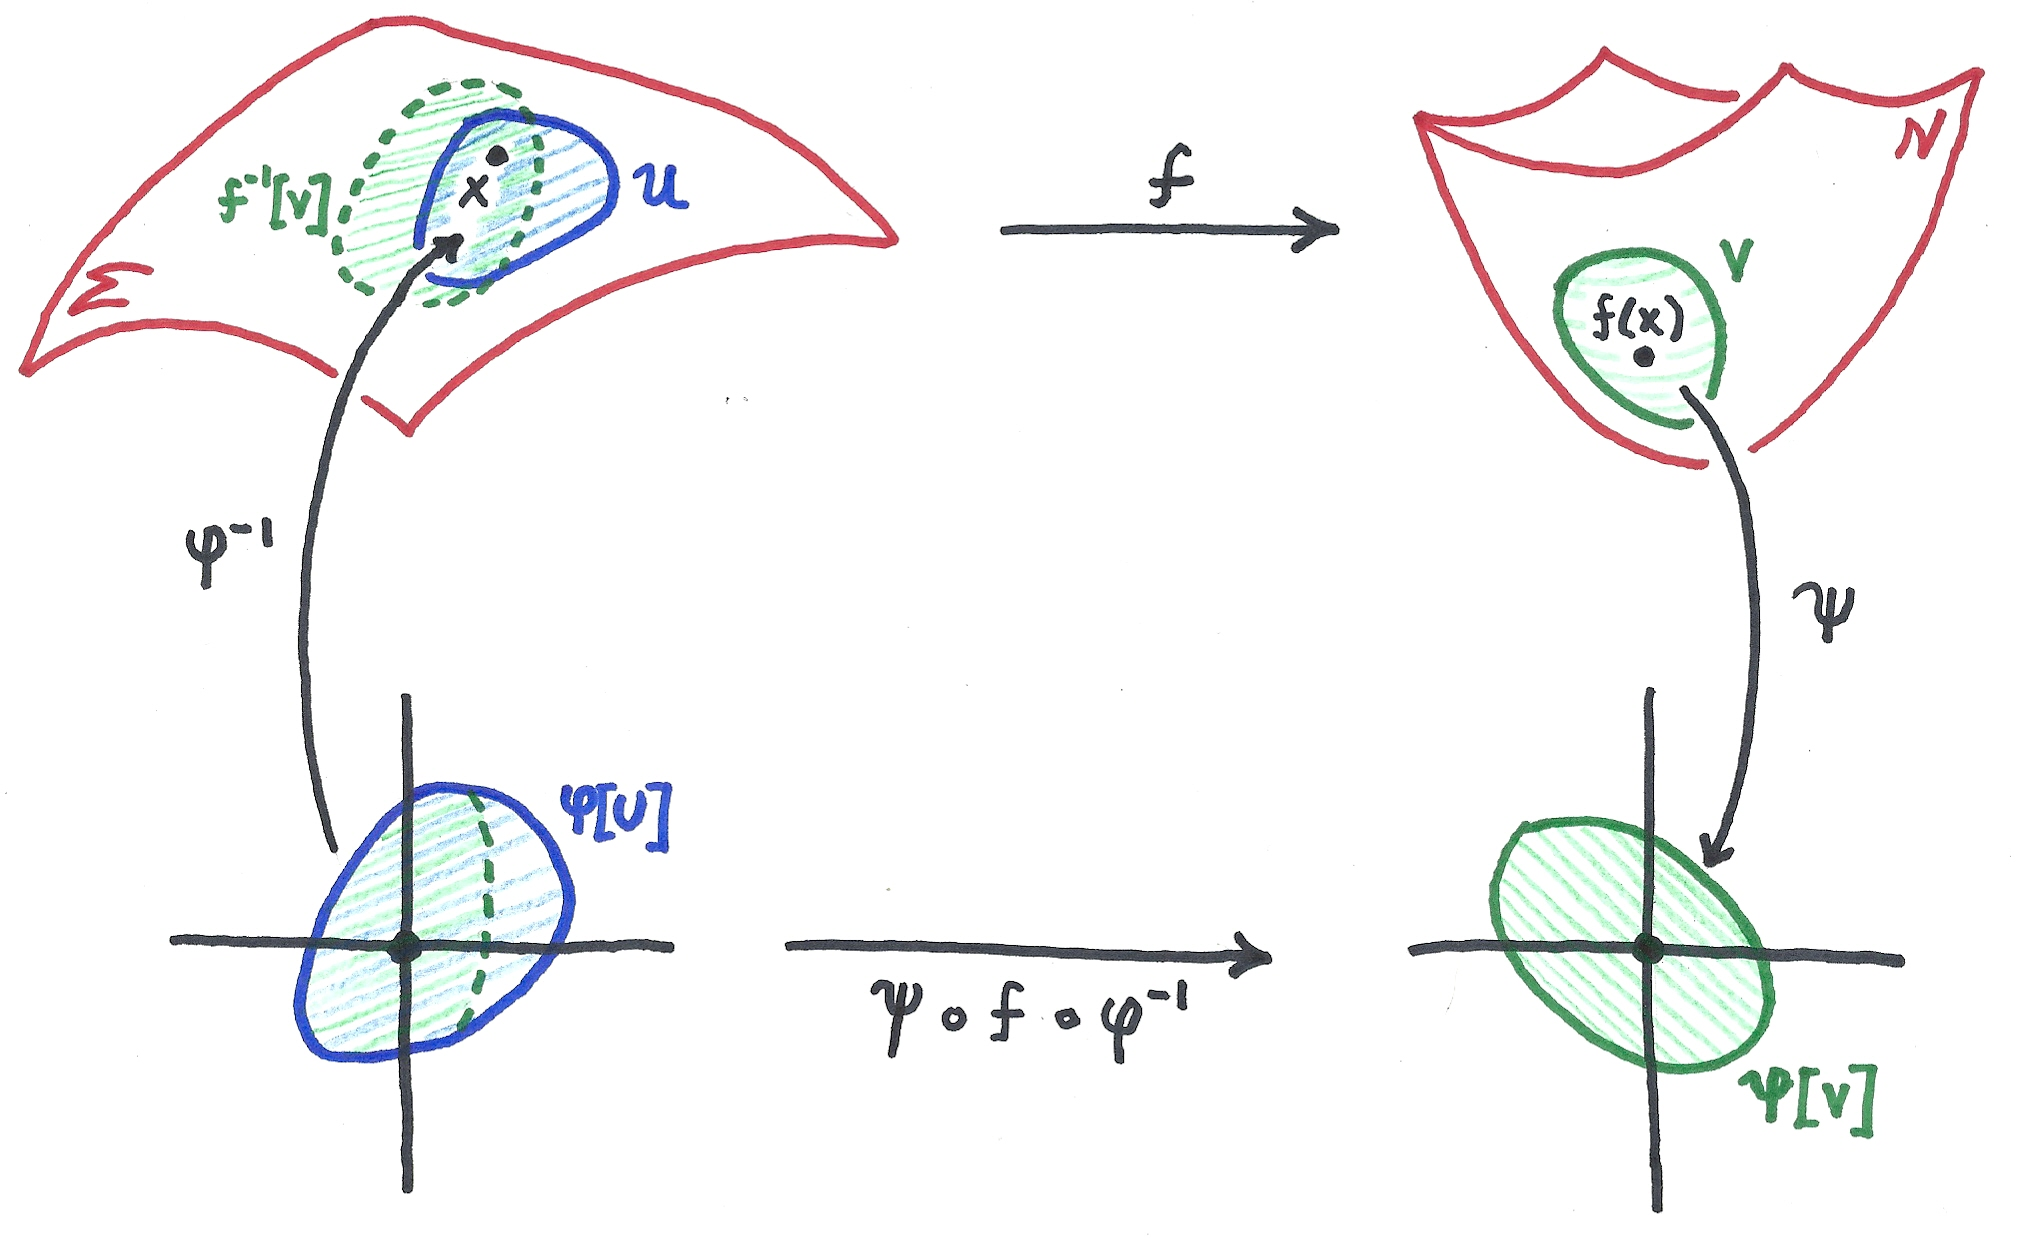
\includegraphics[scale=0.14]{funcion_suave}
  \end{figure}%%%%%%%%%%%%%%%%%%%%%%%%%%%%%%%%%%%%%%%%%%%%%%%%%%%%%%%%%%%%%%%%%%%%%%%%%%

Claramente la categor\'ia $\cat{Var}^{\infty}$ de variedades suaves es una categor\'ia con
las funciones suaves como morfismos. Un isomorfismo en esta categor\'ia se llama
\emph{difeomorfismo} y si existe un difeomorfismo entre dos variedades $M$ y $N$ lo denoto por
$M\cong N$.

\import{\directory}{ejercicios/21} %%%%%%%%%%%%%%%%%%%%%%%%%%%%%%%%%%%%%%%%%%%%%%%%%%%%%% EJERCICIO 21

Es importante notar que la clase de variedades suaves con funciones suaves como morfismos forma una
categor\'ia que llamo $\cat{Variedades}$. Esto se debe a que la identidad $\Id:M\ra M$ siempre es
suave y la composici\'on de dos funciones suaves es suave. Al conjunto de morfismos entre dos
objetos en $\cat{variedades}$ la llamo
\[
    C^{\infty}(M,N) = \Big\{ M\morf{f} N \;\,\big|\;\, f\;\text{es suave}  \Big\}.
\]

En particular el conjunto $C^{\infty}(M,\RR)$ nos dice mucho sobre las propiedades de $M$. Como
$R$ es una variedad suave, $C^{\infty}(\,\cdot,\RR)$ es un funtor contravariante a la categor\'ia
de $\RR$-\'algebra. En efecto:
\[
  (f+g)(x):=f(x)+g(x) \quad\text{y}\quad (fg)(x):=f(x)g(x)
\]
le definen una estructura de anillo conmutativo con 1 a $C^{\infty}(M,\RR)$ y adem\'as, el subanillo
de las funciones constantes es isomorfo a $\RR$ y as\'i $C^{\infty}(M,\RR)$ es un $\RR$-\'algebra.

$C^{\infty}(M,\RR)$ tambi\'en tiene estructura de $\RR$-espacio vectorial, entonces podemos
definir su espacio dual:
\[
  C^{\infty}(M,\RR)^*:=\Big\{ C^{\infty}(M,\RR) \morf{v} \RR \;\,\big|\;\, v\;\text{es lineal} \Big\}
\]


Una vez mencionado esto, defino:

\begin{defin}
  Una \emph{derivaci\'on} en $x\in M$ es un funcional lineal $d:C^{\infty}(M,\RR)\ra\RR$ con
  $f\mapsto df$ que cumple la regla de Liebniz: $d(fg)=g(x)df+f(x)df$. El conjunto de todas
  las derivaciones en $x$ se llama el \emph{espacio tangente} de $M$ en $x$:
  \[
    T_x M:=
    \big\{d\in C^{\infty}(M,\RR)^*\;\big|\;
    d(fg)=g(x)df+f(x)dg \;\;\forall f,g\in C^{\infty}(M,\RR)\big\}
  \]
\end{defin}

Observa que $T_x M$ es un subespacio vectorial de $C^{\infty}(M,\RR)^*$ porque si $d,d'\in T_x M$
y $\la\in\RR$ es un escalar entonces
\begin{align*}
  (d+\la d')(fg)& =
  d(fg)+\la d'(fg) \\ & =
  g(x)df+f(x)dg+\la g(x)d'f+\la f(x)d'g \\ & =
  g(x)(df+\la d'f)+f(x)(dg+\la d'g)\\ & =
  g(x)(d+\la d')(f)+f(x)(d+\la d')(g)
\end{align*}
y $T_x M$ es cerrado bajo combinaciones lineales. Adem\'as es claro que el funcional lineal $0$
cumple la regla de Leibniz.

Tomar derivadas parciales es el primer ejemplo de una derivaci\'on: Sea $M$ una variedad suave y
$x\in M$. Si $(U,\varphi)$ una carta alrededor de $x$ entonces $\varphi:U\ra\RR^n$ y as\'i es de la
forma $\varphi=(x_1,\ldots,x_n)$ donde $x_i\in C^{\infty}(M,\RR)$. Con esto defino el siguiente
funcional lineal:
\[
  \left. \frac{\partial}{\partial x_i} \right|_{x}(f)=
  \frac{\partial(f\circ \varphi^{-1})}{\partial x_i}(\varphi(x))
\]
donde la segunda derivada es la usual de $\RR^n$. El funcional lineal $\partial/\partial x_i|_x$
es una derivaci\'on porque la derivada usual es lineal y como toda carta se puede expresar con
$n$ coordenadas, entonces
\[
  \left\{ \left. \frac{\partial}{\partial x_1} \right|_{x},\ldots,
  \left. \frac{\partial}{\partial x_n} \right|_{x}\right\}
\]
es una base de $T_x M$.

Si considero la categor\'ia de variedades suaves basadas, denotado por $\cat{Variedades}_*$,
parece que $(M,x)\mapsto T_x M$ es un funtor a la categor\'ia de espacios vectoriales sobre $\RR$,
pero para probar esto necesito saber c\'omo transforma este funtor a las funciones suaves
$f:(M,x)\ra(N,y)$.

\begin{defin}
  Sea $F:(M,x)\ra (N,y)$ una funci\'on suave entre variedades suaves basadas. Entonces el
  \emph{diferencial} de $F$ en $x$ lo defino como la funci\'on:
  \[
    D_xF:T_x M \lra T_{y}N \quad\text{con}\quad (D_xF(d))(f)=d(f\circ F)
  \]
\end{defin}

\import{\directory}{ejercicios/23} %%%%%%%%%%%%%%%%%%%%%%%%%%%%%%%%%%%%%%%%%%% EJERCICIO 23

Ahora defino lo necesario para estudiar las 'inclusiones' en la categor\'ia de las variedades
suaves:

\begin{defin}
  Sea $M$ de dimensi\'on $m$ y $N\subseteq M$ un subespacio de $M$. Entonces $N$ es una
  \emph{subvariedad} de dimensi\'on $n\leq m$ si para toda $x\in N$ existe una carta $(U,\varphi)$
  de $M$ alrededor de $x$ tal que:
  \[
    \varphi[U\cap N]=\varphi[U]\cap(\RR^n\times\{0\})\subset \RR^m
  \]
  donde $0\in\RR^{n-m}$.
\end{defin}

El siguiente ejemplo ilustra bien esta definici\'on:
  Si hago $\Sn^1=(\cos 2\pi t,0,\sin 2\pi t)\subset\Sn^2\subset\RR^3$ (mediante el difeomorfismo
  $e^{2\pi i t}\mapsto(\cos 2\pi t,\sin 2\pi t,0)$), entonces las \'unicas cartas que intersectan
  a $\Sn^1$ son $V_1^{\pm}$ y $V_2^{\pm}$, entonces (por ejemplo):
\begin{align*}
  h_i^{\pm}[V_i^{\pm}\cap \Sn^1]& =\left.
  \begin{cases}
      (x_2,x_3)=(\sin 2\pi t,0)\;\; , \;\; t\in[0,1] & \text{si}\;\; i=1 \\
      (x_1,x_3)=(\cos 2\pi t,0)\;\; , \;\; t\in[0,1] & \text{si}\;\; i=2
  \end{cases}\right\} \\ & =
  (-1,1)\times\{0\} \\ & =
  \overset{\circ}{\mathbb{D}}\cap (\RR^1\times\{0\}) \\ & =
  h_i^{\pm}[V_i^{\pm}]\cap (\RR^1\times\{0\}) \quad(i=1,2)
\end{align*}
es decir que $\Sn^1$ es una subvariedad de $\Sn^2$. Similarmente $\Sn^n$ es una subvariedad
de $\Sn^m$ para toda $n\leq m$. El siguiente dibujo ilustra este ejemplo:
  \begin{figure}[ht]%%%%%%%%%%%%%%%%%%%%%%%%%%%%%%%%%%%%%%%%%%%%%%%%%%%%%%%%%%% FIGURA
    \centering
    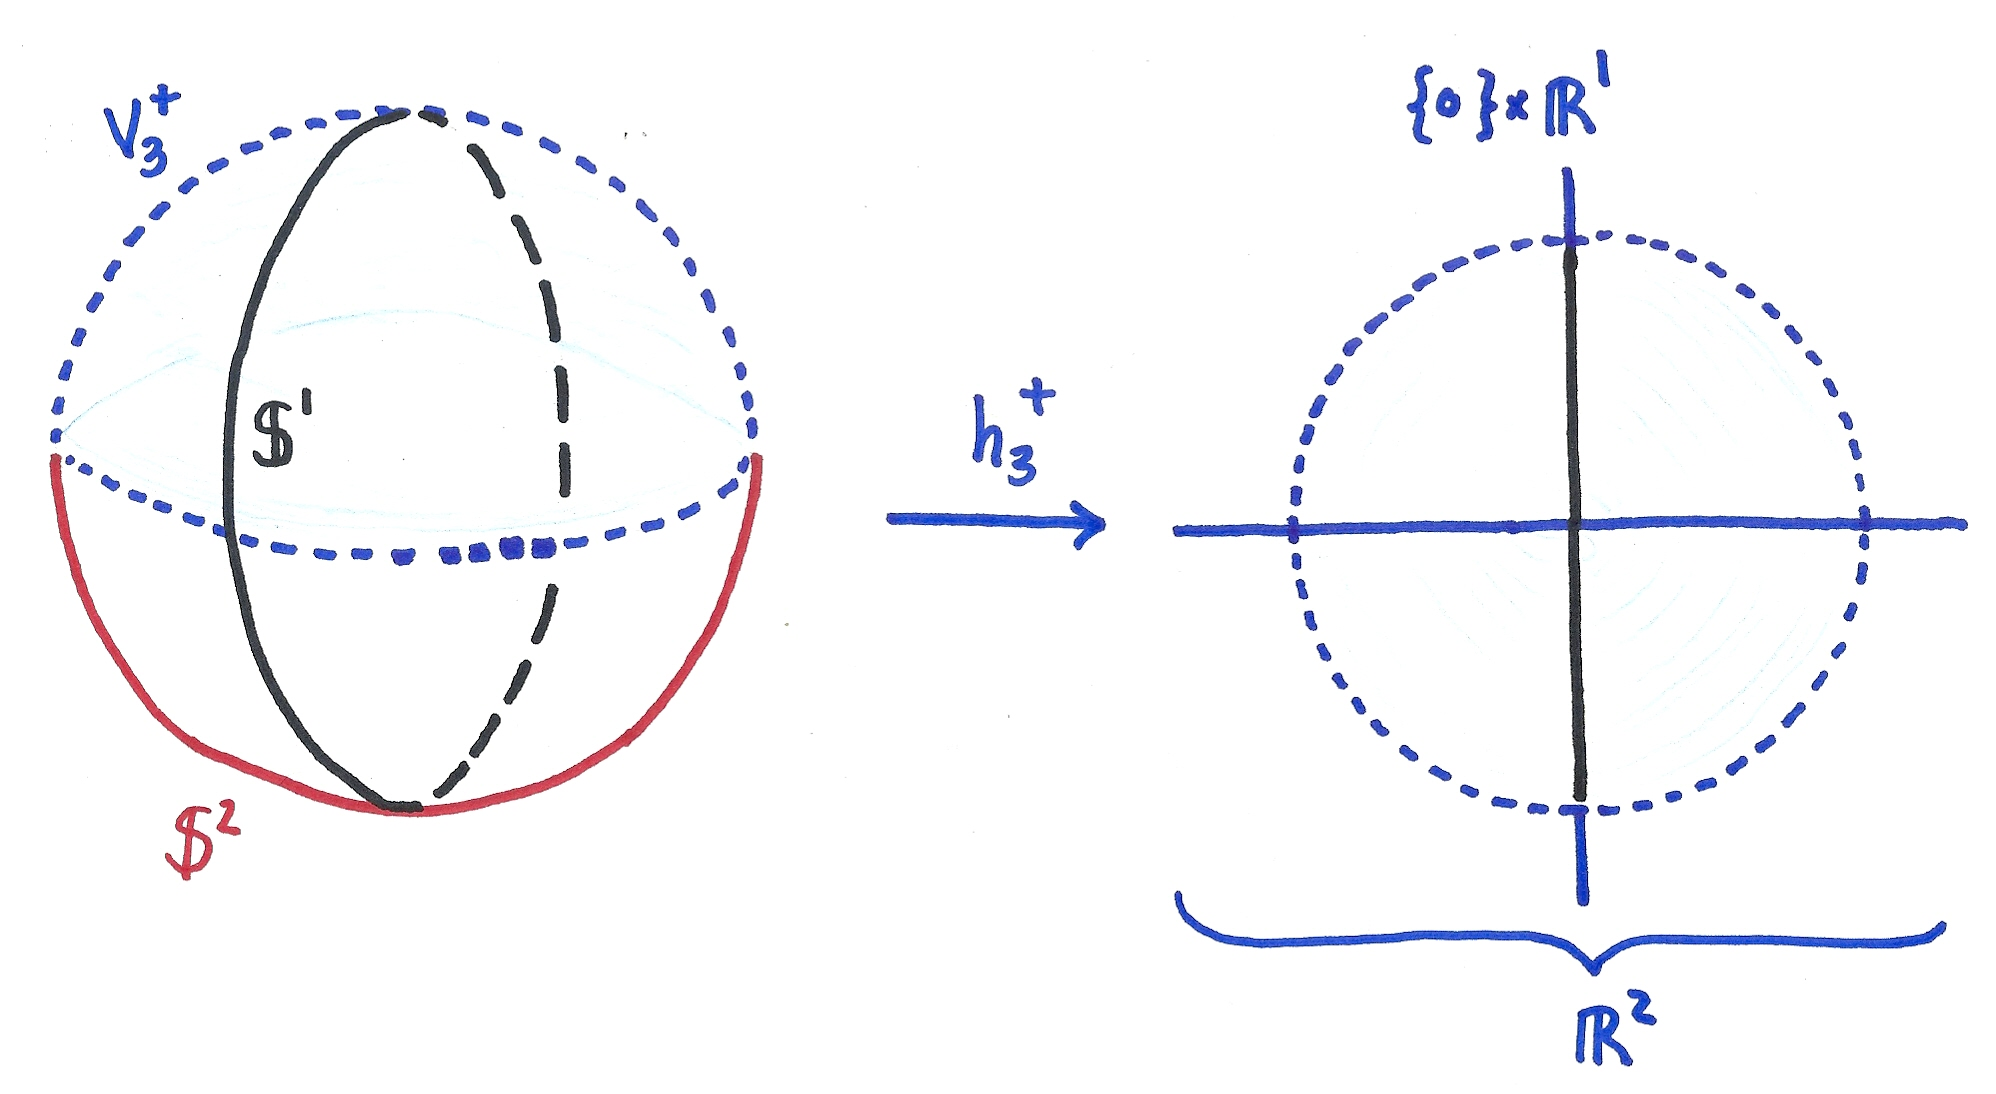
\includegraphics[scale=0.12]{subvariedad}
  \end{figure}%%%%%%%%%%%%%%%%%%%%%%%%%%%%%%%%%%%%%%%%%%%%%%%%%%%%%%%%%%%%%%%%%%%%%%%%%%



Esto sugiere la descripci\'on: una subvariedad $N$ vive en $M$ como
$\RR^n\times\{0\}$ vive en $\RR^m$.

Adem\'as si $\fA=\{(U_{\alpha},\varphi_{\alpha})\}_{\alpha\in A}$
es el atlas suave de $M$, entonces $N$ tiene estructura diferenciable con el atlas restringido
\[
  \fA|_N:=\big\{\big(U_{\alpha}\cap N,(\varphi_{\alpha})|_{U_{\alpha}\cap N}\big)\big\}_{\alpha\in A}.
\]
Con el atlas $\fA|_N$, la inclusi\'on $\iota:N\ra M$ se vuelve suave. Este tipo de inclusi\'on
se generaliza. Si una variedad $N'$ es difeomorfa una subvariedad $N\subseteq M$ (equipada de
su atlas $\fA|_N$), mediante un difoemorfismo $f$, entonces la funci\'on $\iota':=\iota\circ f$
la puedo pensar como una ``inclusi\'on''.

\begin{defin}
  Una funci\'on suave $f:N\ra M$ es un \emph{encaje} si la imagen $f[N]\subseteq M$ es una
  subvariedad de $M$ y adem\'as $N\cong f[N]$. En este caso lo denoto por $N\hookrightarrow M$.
\end{defin}

Por lo tanto para todo encaje $f$ existe una factorizaci\'on $f=\iota\circ f'$ donde $f'$ es el
difeomorfismo $N\ra f[N]$ y $\iota:f[N]\ra M$ es la inclusi\'on. En palabras esto quiere decir
que un encaje $N\hookrightarrow M$ es una transformaci\'on que te permite ver a $N$ como subvariedad
de $M$.

Parece que la definici\'on de encaje es muy restrictiva pero Whitney prob\'o que:

\begin{thm}(Whitney)
  Toda variedad suave de dimensi\'on $m$ se puede encajar en $\RR^{2m}$, es decir para toda
  variedad $M^m$, existe $M\hookrightarrow \RR^{2m}$.
\end{thm}

Este teorema es muy fuerte por varias razones. Primero, esto significa que cualquier variedad la
podemos identificar con una subvariedad de un espacio euclideano. Segundo, la dimensi\'on de este
espacio euclideano se puede minimizar a dos veces la dimensi\'on de la variedad original. Por ejemplo
$\RR P^2\not\hookrightarrow\RR^3$ porque la imagen tendr\'ia que autointersectarse (y as\'i
fallar\'ia la inyectividad). Entonces $2m$ es la m\'inima dimensi\'on necesaria para poder encajar
cualquier variedad en un espacio euclideano.

\begin{defin}
  Sea $f:M\ra N$ una funci\'on suave. Un punto $y\in N$ es un \emph{valor regular} si para todo
  elemento $x\in f^{-1}[\{y\}]$ el diferencial $D_xf$ es sobreyectivo. Si esto no se cumple,
  entonces $y$ es un \emph{valor cr\'itico}.
\end{defin}

La importancia de los valores regulares se muestra con el siguiente teorema:

\begin{thm}\label{thm:imagen_inversa_valor_regular_subvariedad}
  Sea $f:M^m\ra N^n$ una funci\'on suave y $y\in N$ un valor regular. Entonces
  $L=f^{-1}[\{y\}]\subseteq M$ es una variedad de dimensi\'on $m-n$.
\end{thm}

Este teorema y la definici\'on de valor regular se muestra en la figura \ref{fig:valor_regular}:

\begin{figure}[t]%%%%%%%%%%%%%%%%%%%%%%%%%%%%%%%%%%%%%%%%%%%%%%%%%%%%%%%%%%% FIGURA
  \centering
  \label{fig:valor_regular}
  \caption{Los valores regulares y las fibras de la funci\'on altura $\text{ht}:\TT^2\ra\RR$.}
  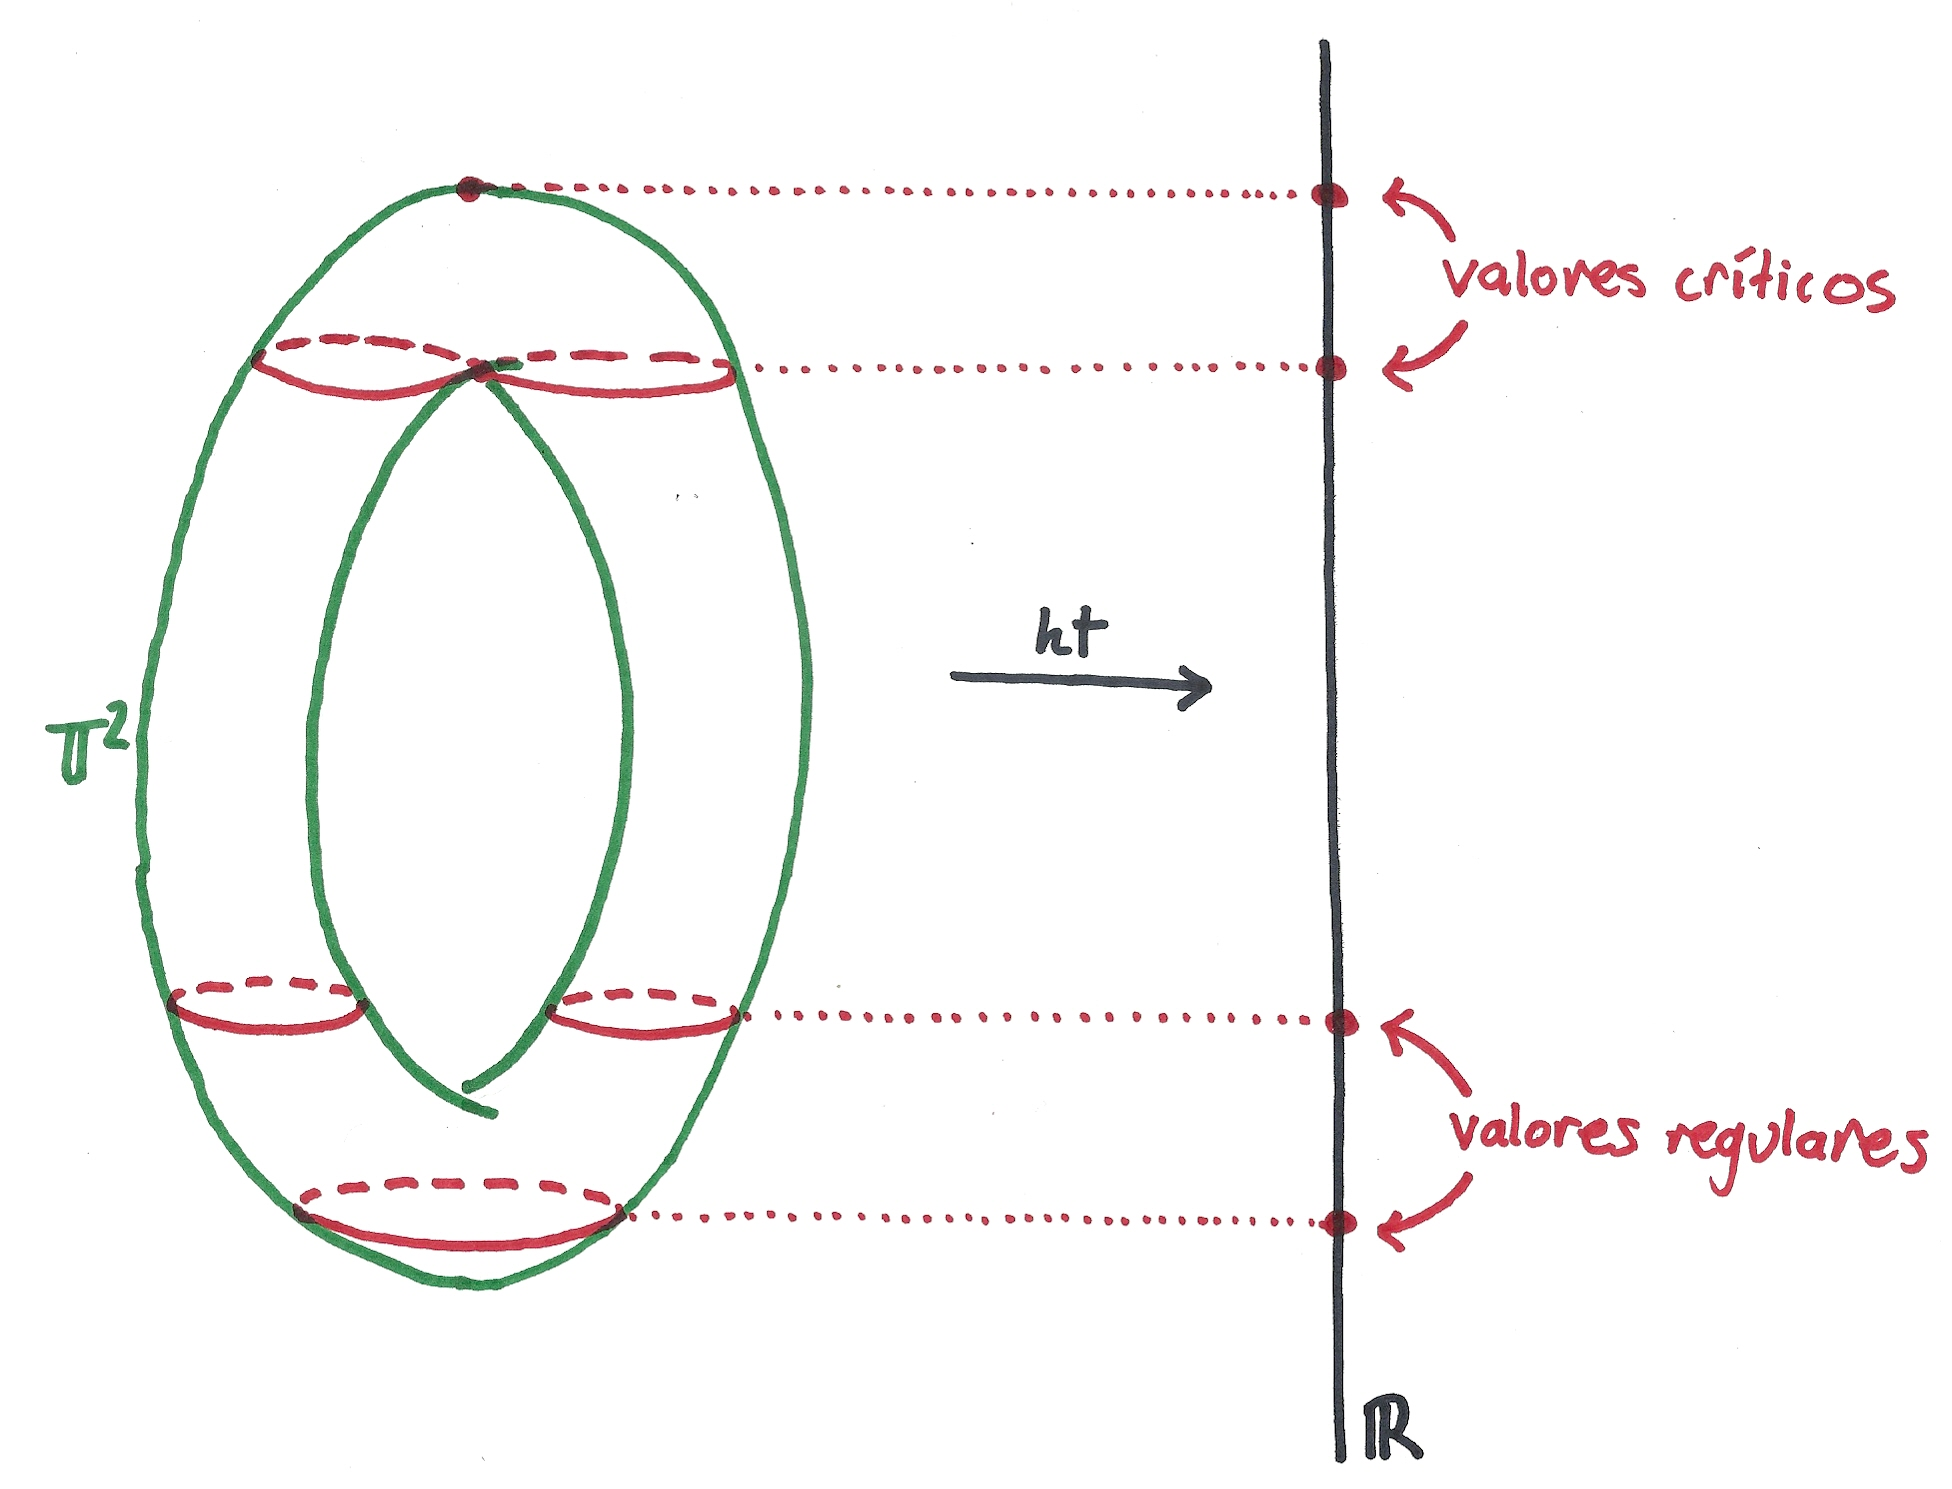
\includegraphics[scale=0.10]{valor_regular}
\end{figure}%%%%%%%%%%%%%%%%%%%%%%%%%%%%%%%%%%%%%%%%%%%%%%%%%%%%%%%%%%%%%%%%%%%%%%%%%%

El famoso Teorema de Sard dice que casi todo valor $y\in N$ es regular: si $C\subset N$ es el
conjunto de puntos cr\'iticos, ie no-regular, de una funci\'on suave $f:M\ra N$,
entonces para toda carta $(U,\varphi)$ de $N$ que intersecta $C$, el teorema de Sard dice
que $\varphi[U\cap C]\subset\RR^n$ es de medida cero.

Con esto defino que cualquier subconjunto $X\subseteq N$ de una variedad es de medida cero
si bajo cualquier carta, su imagen en $\RR^m$ es de medida cero. As\'i enuncio el teorema
de Sard:

\begin{thm}(Sard)
  Sea $f:M\ra N$ una funci\'on suave. El conjunto de valores cr\'iticos es de medida cero.
  En particular el conjunto de valores regulares es denso en $N$.
\end{thm}

Una consequencia importante de este teorema es que se puede calcular el grupo de homotop\'ia:
\begin{equation}\label{eq:pi_m<n}
  \pi_m(\Sn^n,1)=0 \quad\forall m<n
\end{equation}
Si $[\alpha]\in\pi_m(\Sn^n,1)$, claramente $\alpha$ no tiene porque ser suave, pero si lo
fuera, Sard dice que $\alpha:\Sn^m\ra\Sn^n$ tiene un valor regular $y\in\Sn^n$. Ahora si
$x\in \alpha^{-1}[\{y\}]$ entonces $d_x\alpha:T_x\Sn^m\ra T_y\Sn^n$ es sobre, pero esto
nunca puede pasar porque $T_x\Sn^n\cong\RR^n$ y $n>m$. Por lo tanto $f^{-1}[\{y\}]=\emptyset$,
es decir que $\alpha[\Sn^m]\subseteq \Sn^n-\{y\}\subset\Sn^n$.

Co-restrinjo $\alpha:\Sn^m\ra\Sn^m$ a $\alpha':\Sn^m\ra\Sn^n-\{y\}$. Como $\Sn^n-\{y\}\cong\RR^n$
mediante la proyecci\'on estereogr\'afica, entonces $\alpha'\simeq \cte$. Adem\'as, como
$\alpha$ y $\alpha'$ tienen la misma regla de correspondencia: 
\[
  \alpha= \iota\circ\alpha \simeq \iota\circ\cte =\cte
\]
donde $\iota:\Sn^n-\{y\}\hookrightarrow\Sn^n$ es la inclusi\'on. Por lo tanto $[\alpha]=0$.

Acabo de probar que si toda clase de equivalencia $[\alpha]\in\pi_m(\Sn^n,1)$ tiene un representante
$\alpha:\Sn^m\ra\Sn^n$ suave, entonces $\pi_m(\Sn^n,1)=0$. En otras palabras la ecuaci\'on
(\ref{eq:pi_m<n}) se sigue de:

\begin{thm}\label{thm:deformacion_suave}
  Sea $f:M\ra N$ una funci\'on continua (o basada) entre variedades suaves. Entonces existe una
  $f':M\ra N$ suave tal que $f\simeq f'$.
\end{thm}

Otra consecuencia importante del teorema de Sard requiere de orientaci\'on. Primero defino
orientaci\'on para espacios vectoriales y luego lo defino para variedades mediante los
espacios tangentes.

Sea $V$ un espacio vectorial real de dimensi\'on $n$ y denoto por $\fB$ como el conjunto de
todas las bases de $V$. Observa que $\fB$ es isomorfo al espacio de matrices invertibles
$\text{GL}(n,\RR)$. Defino sobre $\fB$ la siguiente relaci\'on:
\[
  \{v_1,\ldots,v_n\}\sim\{w_1,\ldots,w_n\} \quad\iff\quad
  \text{la matriz de cambio de base tiene determinante positivo}.
\]

\import{\directory}{ejercicios/24} %%%%%%%%%%%%%%%%%%%%%%%%%%%%%%%%%%%%%%%%%%%%%%%% EJERCICIO 24

\import{\directory}{ejercicios/25} %%%%%%%%%%%%%%%%%%%%%%%%%%%%%%%%%%%%%%%%%%%%%%%% EJERCICIO 25

Para fines pr\'acticos denoto $\fB/_{\sim}=\{1,-1\}$

\begin{defin}
  Sea $V$ un espacio vectorial real de dimensi\'on $n$. Una \emph{orientaci\'on} de $V$ es la
  elecci\'on de un elemento de $\fB/_{\sim}=\{1,-1\}$.
\end{defin}

\begin{defin}
  Sean $V$ y $W$ espacios vectoriales reales de dimensi\'on $n$ con orientaciones $[\beta]$ y
  $[\gamma]$ (donde $\beta=\{v_1,\ldots,v_n\}$ y $\gamma$ son bases de $V$ y $W$ respectivamente).
  Una transformaci\'on lineal $T:V\ra W$ \emph{preserva orientaci\'on} si
  \[
    T(\beta)=\{T(v_1),\ldots,T(v_n)\}\sim\gamma
  \]
  es decir que la imagen de $\beta$ tiene la misma orientaci\'on que $\gamma$.
\end{defin}

Con estas dos definiciones puedo generalizar orientaci\'on a una variedad:

\begin{defin}
  Sea $M$ una variedad suave. Una \emph{orientaci\'on} de $M$ es una familia $\fO=\{\fo_x\}_{x\in M}$
  donde cada $\fo_x$ es una orientaci\'on de $T_xM$ tal que para toda $x\in M$ existe una carta
  $(U,\varphi)$ de $M$ alrededor de $x$ tal que $D_x\varphi:T_xM \ra T_{\varphi(x)}\RR^n\cong\RR^n$
  preserva orientaci\'on donde $\RR^n$ est\'a orientado can\'onicamente. Una variedad junto
  con una orientaci\'on se llama \emph{variedad orientada} y se denota como la pareja $(M,\fO)$.
\end{defin}

Una vez definido orientaci\'on puedo seguir con otra aplicaci\'on del teorema de Sard:

Quiero analizar la ecuaci\'on (\ref{eq:pi_m<n}) cuando $n=m$. Tomo $[\alpha]\in\pi_n(\Sn^n,1)$
con $\alpha:\Sn^n\ra\Sn^n$ suave (estoy usando el teorema \ref{thm:deformacion_suave}) y $y\in\Sn^n$
un valor regular. Por el teorema (\ref{thm:imagen_inversa_valor_regular_subvariedad}) tengo que
$M_y=f^{-1}[\{y\}]$ es una subvariedad de $\Sn^n$ de dimensi\'on $0$. Observa que $M$ es compacto
(por ser un subconjunto cerrado de un compacto), entonces $M_y=\{y_1,\ldots,y_k\}$ es finito.

Se puede definir una funci\'on $\text{grad}:C^{\infty}(\Sn^n,\Sn^n)\ra\ZZ$ de la siguiente manera:
para $\alpha:\Sn^n\ra\Sn^n$, toma $y\in\Sn^n$ un valor regular. Para cada $x\in M_y=f^{-1}[y]$
calculo
\[
  \text{grad}_{x}(\alpha):=
  \begin{cases}
    +1 & \text{si}\;\; D_{x}\alpha\;\;\text{preserva orientaci\'on} \\
    -1 & \text{si}\;\; D_{x}\alpha\;\;\text{no preserva orientaci\'on}
  \end{cases}
\]
y defino:
\[
  \text{grad}(\alpha)=\sum_{x\in f^{-1}[y]}\text{grad}_x(\alpha)
\]
Para probar que $\text{grad}$ est\'a bien definida necesito probar que no depende del valor regular
$y$ que elig\'i.

\begin{ejemplo}
  Sea $\alpha:\Sn^1\ra\Sn^1$ definido por $z\mapsto z^3$, claramente es suave. Si encajo $\Sn^1$
  en $\RR^2$ como $z=x+iy=(x,y)$, entonces $\alpha$ es la restricci\'on de
  $f(x,y)=(x+iy)^3=(x^3-3xy^2,3x^2y-y^3)$, definido sobre todo $\RR^2$, al c\'irculo unitario.
  Entonces tengo que
  \[
    D_z\alpha=D_{(x,y)}f=3
    \begin{pmatrix}
      x^2-y^2 & -2xy \\
      2xy & x^2-y^2      
    \end{pmatrix}=
    3z^2
  \]
  cuyo determinante es
  \[
    \Delta=(x^2-y^2)^2+4x^2y^2>0  \quad\forall x+iy\in\Sn^1.
  \]
  Esto quiere decir que $D_{(x,y)}$ preserva orientaci\'on en cada punto de $\Sn^1$. Por lo tanto
  en la f\'ormula de $\text{grad}(\alpha)$aparecen puros $+1$'s, es decir
  $\text{grad}(\alpha)=\#\big( \alpha^{-1}[z] \big)$

  Adem\'as $D_z\alpha$
  es claramente sobre ($3z^2$ es una rotaci\'on seguida de una expansi\'on; ambas son funciones biyectivas
  del plano). Por lo tanto todo $z\in\Sn^1$ es un punto regular.

  Por la f\'ormula de de Moivre, sabemos calcular los tres elementos de $x\in\alpha^{-1}[z]$, de hecho
  para cada $z_0\in\Sn^1$ fija, $\alpha^{-1}[z_0]$ es simpliemente las raices del polinomio $z^3-z_0$
  y por el teorema fundamental del \'algebra tiene 3 raices (contando multiplicidad). Por la f\'ormula de
  de Moivre, sabemos que son tres raices distintas:
  \[
    \alpha^{-1}[z]=\left\{ e^{2\pi it/3},e^{2\pi i(t+1)/3},e^{2\pi i(t+2)/3} \right\}.
  \]
  Por lo tanto el grado de $\alpha$ est\'a bien definido para cualquier valor regular y vale
  $\text{grad}(\alpha)=3$. Esto sugiere la idea de que $\alpha$ enrollar el c\'iruclo tres veces:
\end{ejemplo}

\begin{thm}(Hopf)
  La funci\'on $\text{g}:\pi_n(\Sn^n,1)\ra\ZZ$ es un isomorfismo de grupos, es decir:
  \[
    \pi_n(\Sn^n,1)\cong\ZZ
  \]
\end{thm}

\subsection{Variedades con frontera}

Es \'util introducir variedades con frontera, especialmente para la secci\'on \ref{sec:cobordismo}.
La definici\'on es casi id\'entica a la definici\'on usual de variedad, pero antes de empezar s\'olo
recuerdo que el semiplano $\HH^n\subset\RR^n$ se define como
$\HH^n=\{(x_1,\ldots,x_{n})\in\RR^n\mid x_n\geq 0\}$.

\begin{defin}
  Sea $M$ un espacio topol\'ogico paracompacto. $M$ es una \emph{variedad con frontera} si para
  todo $x\in M$ existe una vecindad abierta $U$ de $x$ y una funci\'on continua $\varphi:U\ra\HH^n$
  que es un homeomorfismo sobre su imagen. La \emph{frontera} de $M$ se define como
  $\partial M:=\{x\in M\mid \exists (U,\varphi)\;\text{tal que}\;\varphi(x)=(x_1,\ldots,x_{n-1},0)\}$
  \begin{figure}[ht]%%%%%%%%%%%%%%%%%%%%%%%%%%%%%%%%%%%%%%%%%%%%%%%%%%%% FIGURA VARIEDAD_CON_FRONTERA
    \centering
    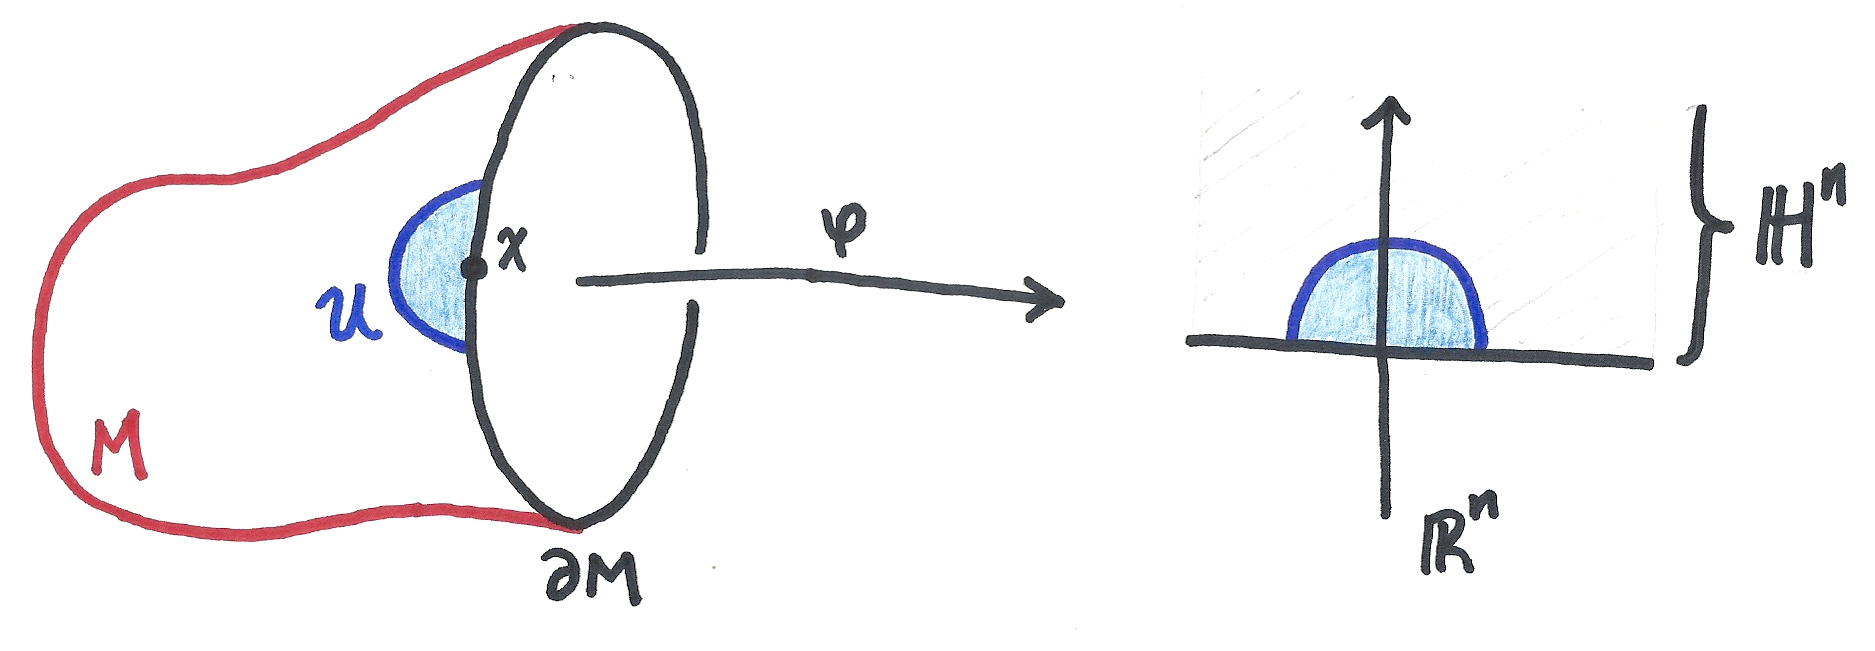
\includegraphics[scale=0.12]{variedad_con_frontera}
  \end{figure}%%%%%%%%%%%%%%%%%%%%%%%%%%%%%%%%%%%%%%%%%%%%%%%%%%%%%%%%%%%%%%%%%%%%%%%%%%%%%%%%%%%%%%%
\end{defin}

\noindent Ojo: probar que $\partial M$ est\'a bien definido es muy complicado

\begin{nota}
  De ahora en adelante ``variedad'' siempre significa una variedad sin frontera como en la definici\'on
  original y ``variedad con frontera'' siempre se refiere a la definici\'on anterior.
\end{nota}

La frontera $\partial M$ de una variedad con frontera $M^n$ es naturalmente una variedad de
dimensi\'on $n-1$, entonces viene equipado de un espacio tangente $T_x\partial M$ para cada
$x\in \partial M$. Adem\'as, $x\in \partial M\subset M$ tambi\'en tiene asociado el espacio tangente
$T_xM$. Por lo tanto $T_x\partial M$ es un subespacio de $T_xM$ de codimensi\'on 1 y as\'i, divide
el espacio tangente en dos semiplanos.

Dado un vector $v\in T_xM-T_x\partial M$, \'este puede estar en s\'olo uno de estos semiplanos.
Decimos que $v$ \emph{apunta hacia adentro} si la variedad $M$ est\'a en la direcci\'on de $v$
y decimos que $v$ \emph{apunta hacia afuera} en el otro caso (ve la siguiente figura).

La orientaci\'on de una variedad se puede traducir a una variedad con frontera. Sea $M$ una variedad
con frontera y supongo que tiene una orientaci\'on $\fO_M:=\{\fo_x\}_{x\in M}$. Entonces puedo
definir una orientaci\'on para $\partial M$ de la siguiente manera:

Para $x\in\partial M\subset M$, tomo la orientaci\'on $\fo_x=[\beta]$ donde $\beta=\{v_1,\ldots,v_n\}$
es una base de $T_xM$ de tal manera que $v_1$ es un vector que apunta hacia afuera. Entonces defino
la orientaci\'on $\fo'_x\in\fO_{\partial M}$ como $\fo'_x=[\{v_2,\ldots,v_n\}]$.
\begin{figure}[ht]%%%%%%%%%%%%%%%%%%%%%%%%%%%%%%%%%%%%%%%%%%%%%%%%%%%%%% FIGURA ORIENTACION_FRONTERA
  \centering
  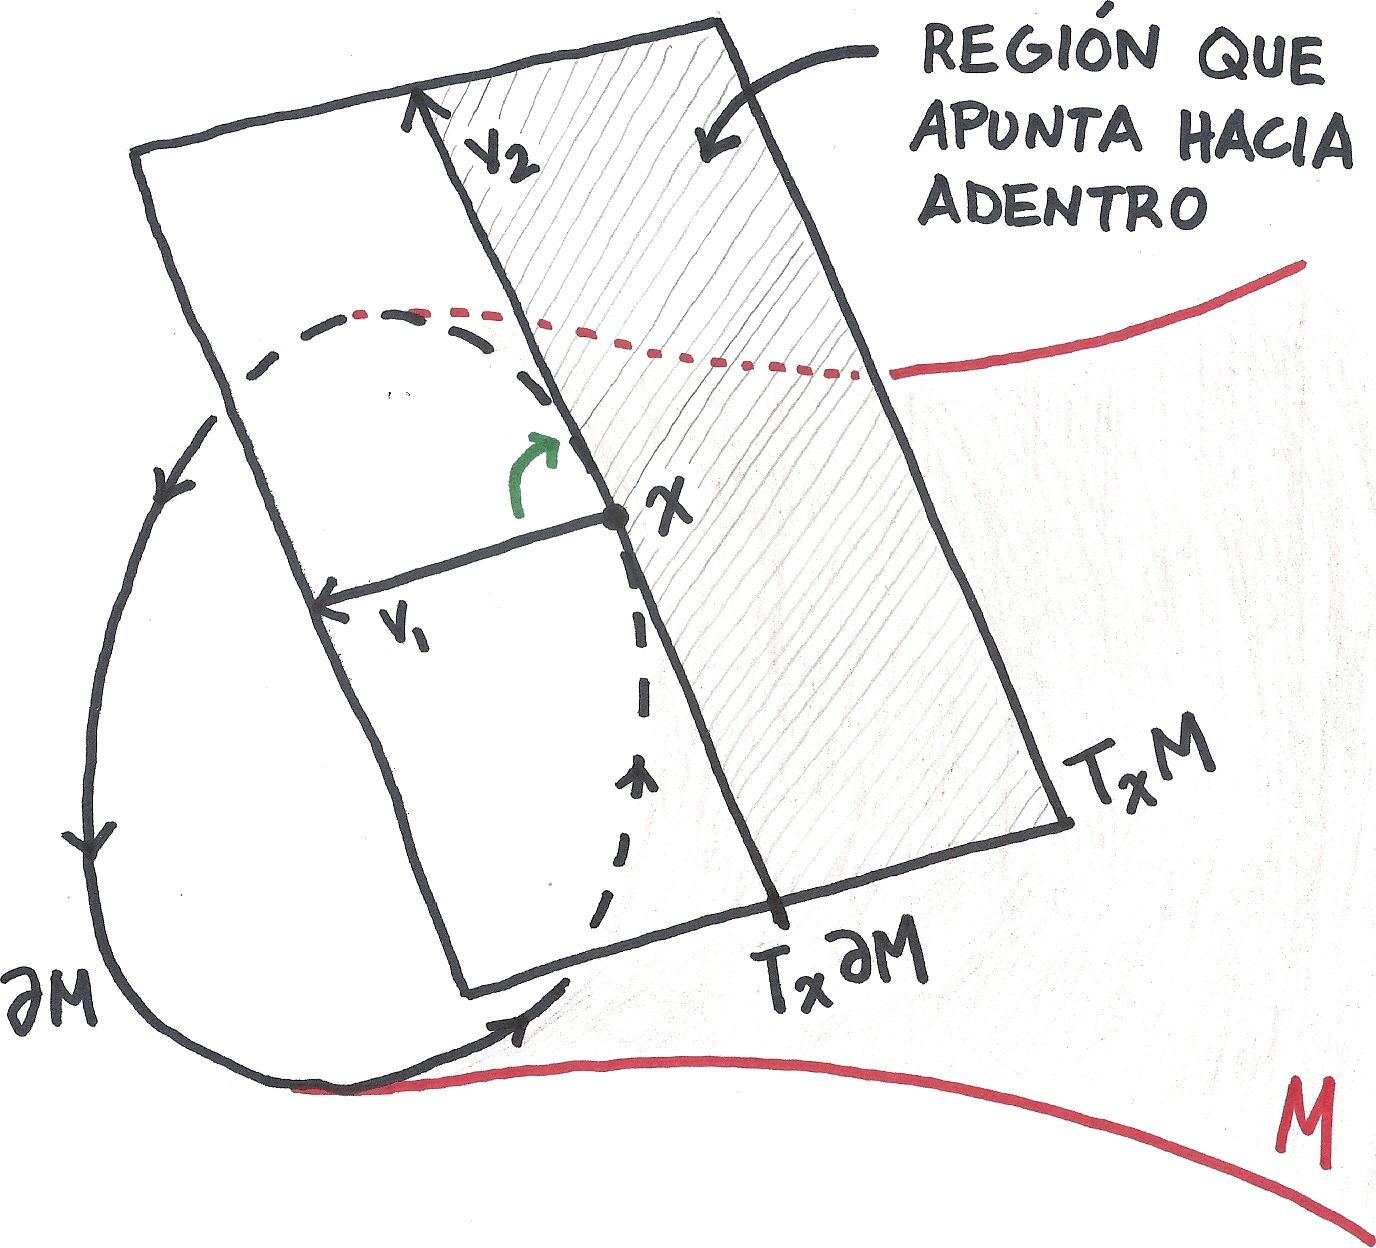
\includegraphics[scale=0.15]{orientacion_frontera}
\end{figure}%%%%%%%%%%%%%%%%%%%%%%%%%%%%%%%%%%%%%%%%%%%%%%%%%%%%%%%%%%%%%%%%%%%%%%%%%%%%%%%%%%%%%%%%
\end{document}